% !TeX root = repressed-anger.tex

\section{Emotion Detection}
\label{sec:emotion_detection}

Emotion detection has been always a important field of study in neuroscience and psychology. Several experiments have been conducted to recognize emotions from face expressions, voice and body gestures, such in \cite{bassili1979emotion}; \cite{banziger2009emotion} and \cite{gunes2007bi}. However, these features are not always available and thus, the detection of emotion from text has gain relevance during the last decade.

Emotion detection from text documents is closely related to \acrshort{sa}. As explained in \ref{subsubsection:sentiment_classification}, sentiment classification task consists in determine the polarity of a given text into two or more classes. Emotion detection also fits this description, since this field of study is conducted by classifying a given document into predefined emotion labels. The definition of these labels are based on previously presented emotion models, which consist on application psychological and neuroscientific theories to represent emotions. One of the first model defined was proposed by Paul Ekman, on 1972, composed by six basic emotions, ``happiness, sadness, fear, anger, surprise and disgust'', and has been used in multiple face recognition systems and is the base emotion detection from text \cite{StevenEmotion2011Classification} as its definition has resulted to be the most semantically diverse \cite{bann2013conceptualisation}.

\begin{figure}[!htp]
  \center
  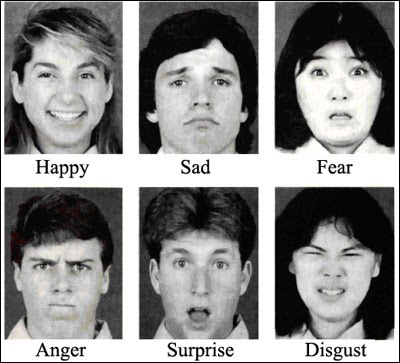
\includegraphics[width=0.5\textwidth]{figures/emotions_ekman}
  \caption{Ekamn's basic emotions, image extracted from Expressions, Emotions and Emblems, Google Sites.}
  \label{fig:ekman_basic_emotions}
\end{figure}

Since then, more interpretations have been made regarding the representation of the emotions, Ekman himself added his list 11 new emotions stating that not all of them could be represented by facial expressions. In 1980 Robert Plutchik TODO

\iffalse
In this section, we will briefly mention Ekman’s emotion model and the OCC (Ortony/Clore/Collins) model. Emotion models stipulate needed knowledge to appraise events. Ekman’s emotion model consists of “sadness, happiness, anger, fear, disgust and surprise” [4]. It has been used in systems that recognise facial expressions related to these emotional states. The OCC model presents emotions generally expressed by an agent. It includes 22 emotion categories [1] designed to model humans in general. It is based on the premise that emotions “are not themselves linguistic things, but the most readily available non phenomenal access we have to them is through language” [1].

The major benefit of using the OCC model is that it provides a specification for different kinds of emotions with a relatively culture free footing. This eliminates the need to study emotions based on specific words but as classes of underlying emotion types. In other words, it is a theory of emotions and not a theory of the language of emotions. The six emotion types in Ekman’s model appear in the OCC model because the specific keywords specified in the former model can be mapped onto specific emotion types specified using tokens (e.g. happiness, sadness, anger, disgust, surprise and fear) in the latter. The OCC emotion types are: Happy-for, Sorry-for, Resentment, Gloating, Hope, Fear, Fears-confirmed, Relief, Disappointment, Pride, Self-Reproach, Appreciation, Reproach, Gratitude, Anger, Gratification, Remorse, Liking, Disliking, Shame, Admiration, Pity[1].
\fi

\cite{binali2010computational}

TODO